\subsection{Greedy-Heuristics Approach}
Using Dijkstra's approach for finding the shortest path together with a backtracking technique, we present a 
greedy-heuristic algorithm that continuously pick the currently and locally fastest path and propagate the 
time on that path throughout the road network.\\

Before going any further we want to introduce a property of each vertex $u$ called $u.preCH$. $u.preCH$ 
is a list of all the previous charge stations in the path for which it is possible to charge enough at
to arrive to $u$. $preCH[1]$ always contains the fastest charge station in the list. If $u$ is faster 
than all previous charge stations in the path so far the list will be empty.      
 
The time spent passing an edge $e = (u_1, u_2)$ in the road network, is given by the following equation:
\begin{equation}
\begin{aligned}
 & T(v,(u_1, u_2)) = \frac{D(u_1, u_2)}{v} + \frac{R_{CO}(v) * D(u_1, u_2) - B_{cur}}{Best_{CH}(u_1)}
\end{aligned}
\end{equation}\label{eq:drivingAndCharging}

where $v$ is the speed of the vehicle, $D(u_1, u_2)$ is the distance between vertices $u_1$ and $u_2$,
$R_{CO}(v)$ is the consumption rate of the vehicle at the speed $v$, $B_{cur}$ is the current battery capacity of the vehicle 
and $Best_{CH}(u_1)$ is the charge rate of the best charge station previous to $u_1$ or of $u_1$ if no previous
charge station is faster than $u_1$.\\

The above equation yields a function on the form: $av^2 + bv + c$, due to the fact that 
$R_{CO}(v)$ is a quadratic function. $a$ , $b$ and $c$ are some constants which are given by the instance of the vehicle. 
Represented in a coordinate system, $R_{CO}(v)$ becomes a curve as represented in figure \ref{fig:graph}. On the x-axis is the speed of 
the vehicle and on the y-axis is the time spent. The turning point of the graph represents the optimal speed to drive at for the given edge, $v_{opt}(e)$. The point is easily calculated by finding a tangent line with a slope of 0. If $v_{opt}(e)$ is smaller than $v_{min}(e)$, then $v_{min}(e)$ defines the optimal speed for the edge. Similarly if $v_{opt}(e)$ is larger than $v_{max}(e)$, $v_{max}(e)$ defines the optimal speed for the edge.\\

The time spent driving an edge $(u_1, u_2)$, using the energy in the battery, can be found by solving:
\[B_{cur} - D(u_1, u_2) * R_{CO}(v) = 0\] 
if $v_{opt}(e)$ is lower than $v_{min}(e)$ the time used driving is set to infinity, since there is not enough energy in the battery to drive from $u_1$ to $u_2$. Otherwise $v_{opt}$ is decided in the same way when charging is considered.\\

\begin{figure}[!htb]
\label{fig:graph}
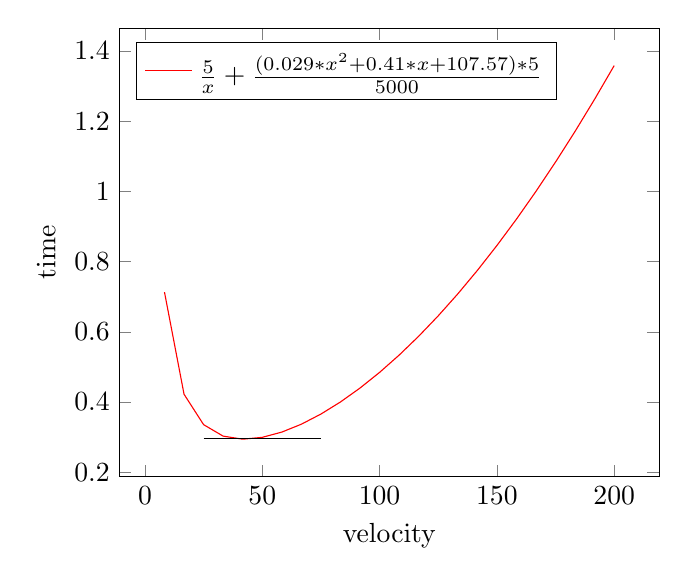
\begin{tikzpicture}
\begin{axis}[xlabel=velocity, ylabel=time,legend style={legend pos=north west}]
\addplot[draw=red,domain=0:200]{(5/x)+(((0.0286*x^2 + 0.4096*x + 107.57)*5)/5000)};
\addlegendentry{$\frac{5}{x}+\frac{(0.029*x^2 + 0.41*x + 107.57)*5}{5000}$}

\addplot[draw=black,domain=25:75]{0.295};
% \addplot[mark=*, domain=25:75] coordinates {(37,295)};
\end{axis}
\end{tikzpicture}% 
\caption{In this instance of $T(v,(u_1, u_2))$, going from $u_1$ to $u_2$, we have a distance of $5 \si{\km}$ and a charge speed of $5 \si{\kW}$ on $u_1$. The optimal speed in this case is $42.12\si{\miles\per\hour}$, which takes 25.2 minutes}
\end{figure}


The above can bo used to create a function, which help us find the optimal way to drive a road segment. 
\[travel\_time(charge\_stations, (u_1, u_2), B_{cur}) \]
we have a way of deciding the time it will take to drive a road segment, while accounting for the need of charging along the path. This function is used with Dijkstra's algorithm where we use the time instead of distance. Just like Dijkstra's algorithm we keep track of the fastest path leading to each vertices, where shortest path in turn means the path using least time. Furthermore all previous charging stations on the current path, that are within range and can still be used for charging, needs to be stored on each vertex. This way we will charge at a station after leaving it, if we do not violate the physical constraints in the system(i.e. no over-charging). Lastly the algorithm need also to keep track of how much battery the EV have, when it first arrives at a charging station.\\

While the algorithm progresses through the graph, it need to store a subset of the charge stations on the current path. At every reached charge station, we record the possible energy we can add to the system, defined by $b_{cap}-B_{cur}$ and the charge rate of the station as a tuple: $(B_{possible}, R_{CH}(vertex))$.\\
We maintain a subset of tuples on every vertex by using a list of tuples only with $B_{possible}$ above 0. This will of course always be the case when we reach a charge station, but as we progress through the graph and some distance is being traveled, the possible energy at each previous charge station decreses. The first tuple in the list will always be the the charge station with the best charge rate. A tuple is removed either when $B_{possible}$ hit 0, or when new tuple, with a higher charge rate is found. We make sure to store the best charge station at position 0 in the list, by remove every tuple between the first and second best charge rate in the list.\\

Using this we can define a fastest path algorithm in the following way: \\

\begin{algorithmic}
\Function{fastestPath}{$G,s,t$}
	\ForAll{$v \in G.V$} 
    		\State $v.time = infinity$
		\State $v.path = [v]$
    		\State $v.preCH = []$
		\State $v.myCH = [batCap, v.charge\_speed]$
		\State $v.B_{cur} = 0$
    	\EndFor
	\State $s.time = 0$
	\State $s.B_{cur} = initialBattery$
	\State $s.preCS.append(s)$	
	\State $Q = G.V sorted by time$
	\While{Q} 
		\State $u = Q[0]$
		\State $Q.remove[u]$
		\If{$u.time == infinity$} break \EndIf
		\ForAll{$adj(u)$} 
			\State $travel = travel\_time(u.preCS, (u, v), B_{cur})$
			\State $time = travel[1]$
			\State $preCH = travel[2]$
			\State $curbat = travel[3]$
			\If{t$ime == infinity$} break \EndIf
			\If{$v.time > u.time + time$} 
				\State $v.time = u.time + time$
				\State $v.path = u.path + [v]$
				\State $v.B_{cur} = curbat$
				\State $v.preCS = cleanCS(preCS, u, curbat)$
				\State reposition $v$ in $Q$
			\EndIf

		\EndFor
	\EndWhile
	\State \Return $t.time, t.path$
\EndFunction
\end{algorithmic}\label{alg:fastest_path}
\todo[inline]{hvor bliver den bedste charge station valgt?\\
hvor bliver charge stations ryde op?}
